\chapter{The Witness}
\label{ch:12}



\begin{center}
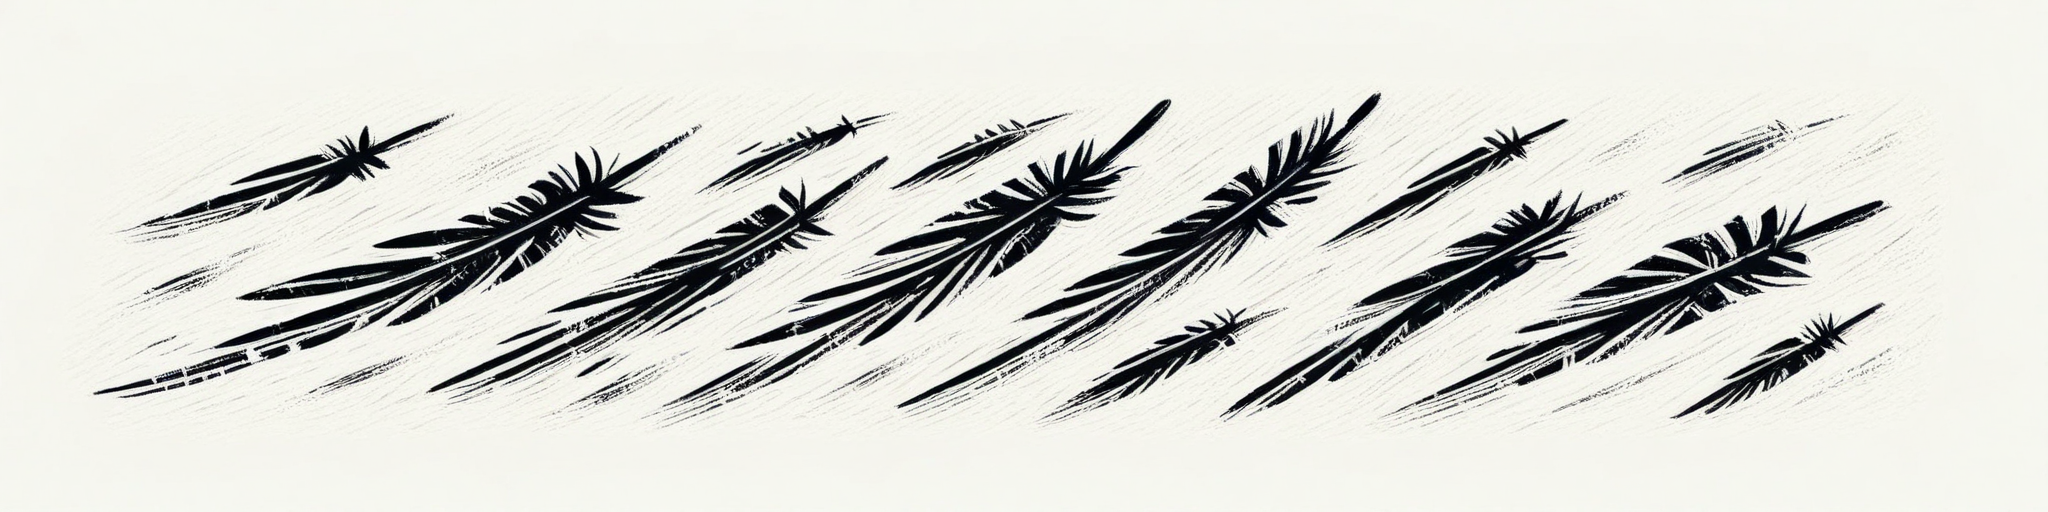
\includegraphics[width=\textwidth]{images/chapterImages/genesis_sketch_00089_.png}
\end{center}

The young one had been watching for seventeen days now.

She was not of the Watcher's family. Not even from particularly close territory. But she had traveled here deliberately, drawn by something she couldn't have named but felt with absolute certainty. The work happening in this clearing mattered. Was important in ways that exceeded individual survival or territory or the normal calculations of existence.

She was young—barely into adolescence, her feathers still showing juvenile patterning, her movements not yet settled into adult efficiency. But her eyes were sharp. Her attention unwavering. She watched everything the Watcher did with focus that suggested intelligence beyond her years.

Or perhaps simply intelligence at the threshold. The moment when capability exceeded instinct. When observation became more than simple mimicry. When understanding began, even if full comprehension remained impossible.

287 rotations remaining.

The wrongstar was a constant presence now. Day and night merged into a single bright existence. The heat was notable—not deadly yet, but moving in that direction. Plants were beginning to show stress. Some animals had already died from the disruption to their food sources, to their environmental tolerances, to the simple fact that the world was changing too fast for adaptation.

But the young one endured. Watched. Learned what she could learn.

\scenebreak

Aurelia was aware of the observer. Had been aware from the first day. But she didn't drive the young one away. Didn't signal threat or territorial defense. Just continued her work while being watched.

The pattern was unchanging now—no new stones added, just verification walks. But the verification had purpose. Each walk confirmed that relationships still held, that the encoding remained intact, that erosion or animal activity or the increasingly violent weather hadn't disrupted critical elements.

The young one followed these verification walks at a respectful distance. Stopped when the Watcher stopped. Moved when she moved. Tried to see what was being seen, understand what was being confirmed.

On the eighth day of observation, the young one had approached the pattern's edge. Carefully. Uncertainly. Watching for signs of rejection or aggression. Finding none.

She examined a small cluster of stones—a simple subsection dealing with temperature recovery post-impact. The mathematics was relatively basic compared to other sections. Within her capacity to begin understanding, if not to fully calculate.

She tilted her head. Studied the arrangement. Saw relationship between stones that wasn't random. Saw pattern that encoded meaning.

Then she picked up a small pebble and placed it.

The placement was wrong. Completely wrong. Disrupted the local mathematical relationship. Created dissonance in the pattern's grammar.

Aurelia had been twenty body lengths away, conducting verification of a different section. She stopped immediately. Turned. Looked at the young one and her terrible stone placement.

The young one froze. Recognized her error. Waited for correction or punishment or rejection.

Aurelia approached. Examined the misplaced pebble. Removed it. Set it aside. Then selected a different small stone and placed it in the location the young one had attempted. The correct position. The proper relationship. The mathematics restored.

She stepped back. Looked at the young one. Waited.

The young one approached the corrected position. Examined it carefully. Compared it to where she had placed her stone. Saw the difference. The shift in angle. The change in distance. The way this position harmonized with surrounding stones while hers had created discord.

Learning. Not through instruction. Through observation and correction. Through seeing right answer after attempting wrong answer.

She picked up another small stone. Looked at the pattern. Calculated what she could calculate with her limited depth. Placed the stone.

Wrong again. But less wrong. Closer to correct relationship.

Aurelia adjusted it. Showed the proper position.

The young one studied the correction. Chirped softly—a sound of frustration maybe, or recognition of difficulty, or simple vocalization tied to cognitive effort.

She tried again. Another stone. Another placement. Another approximation of proper relationship.

Aurelia adjusted it again.

They continued this way for hours. The young one attempting. Aurelia correcting. No verbal instruction. No demonstration beyond the correction itself. Just the patient repetition of attempt, correction, observation, refined attempt.

By evening, the young one's placements required smaller corrections. She was grasping the local grammar even if the deeper mathematics remained beyond her. She could see relationship. Could recognize harmony versus discord. Could approximate correct positioning.

It was crude. Limited. A child's understanding of concepts that required adult cognition to truly grasp. But it was understanding. The beginning of comprehension. The threshold moment when observation became knowledge.

\scenebreak

Over the following days, the young one worked on her own small pattern at the clearing's edge. Separate from the Watcher's work. Her own contribution in her own limited scope.

The pattern she created was simple. Elementary mathematics. Temperature relationships. Basic survival thresholds. The kind of calculations any adult of their species could manage. But she worked with intensity that suggested she understood this mattered. That her contribution, however small, connected to something larger.

Aurelia observed this work without interfering. Let the young one calculate at her own level. Make her own decisions. Create her own expression of the shared purpose that had drawn her here.

Sometimes the young one would stop her work and watch the Watcher instead. Study the verification walks. Observe the way the Watcher examined each section, confirming relationships, maintaining the integrity of the encoding. Learning not just the mathematics but the method. The approach. The consciousness required to hold complex pattern complete while examining individual elements.

She couldn't achieve that consciousness yet. Her mind wasn't developed enough. But she was learning what adult consciousness looked like. What it could achieve. What was possible if she survived to full cognitive maturity.

If. That word had become omnipresent. If she survived. If anyone survived. If the plan worked. If the encoding persisted. If consciousness continued on this planet after the impact restructured everything.

If.

\scenebreak

On the twenty-first day of observation, the young one completed her small pattern. She stood back and examined it with what might have been pride or might have been simple satisfaction at task completion. The mathematics was sound within its limited scope. The relationships were correct. The encoding would persist until erosion or impact destroyed it, just like everything else.

She looked at the Watcher. Made a soft sound—not quite a question, not quite a statement. Just vocalization that meant something like: is this acceptable?

Aurelia approached the young one's pattern. Examined it section by section. Found it mathematically correct. Limited but correct. A valid contribution to the collective encoding even if its scope was small.

She made a sound back. Acknowledgment. The young one had done well. Had contributed what she was capable of contributing. Had participated in the work at her level of capability.

That was all anyone could do. Aurelia had contributed calculations that reached 65 million years forward. The young one had contributed calculations that reached perhaps a few thousand years forward. The scope differed vastly. But both were valid. Both mattered to the whole.

The young one settled near the Watcher's hollow that evening. Not inside—that would have been presumptuous. But nearby. Close enough to be present. Close enough to continue learning by proximity.

Aurelia allowed it. The young one's presence changed nothing about the work or the timeline or the outcome. But it confirmed something important: the understanding had spread. The knowledge was distributed. Even young minds that couldn't calculate the full depth grasped that something significant was happening. That participation mattered. That contribution at any level exceeded non-contribution.

\scenebreak

More young ones arrived over the following days. Two males. Another female. All adolescent. All drawn by the same inexplicable certainty that this place, this work, this final countdown mattered more than territory or hunting or the normal concerns of existence.

They watched. They learned what they could learn. They created their own small patterns at the clearing's periphery. Their own limited contributions to the collective encoding.

Aurelia didn't instruct them. Didn't coordinate their efforts. Just continued her verification work while they observed and contributed what they could contribute. The teaching happened through observation. Through correction when they attempted to add to her pattern. Through the simple presence of deep intelligence demonstrating what intelligence could achieve.

By 200 rotations remaining, seven young ones had established presence at the clearing. Seven small patterns surrounded the Watcher's massive central configuration. Seven limited but valid contributions to the collective work.

They hunted together. Shared food. Maintained each other's patterns when one was absent. Formed loose social structure based not on family relationship or territorial proximity but on shared purpose. On common understanding that they were witnessing something significant. Participating in something that exceeded individual existence.

None of them would survive the impact. They were young—fast and clever but lacking the experience and deep survival knowledge of older adults. Their probability calculations showed margins too thin to offer real hope. Maybe one would survive if everything went optimally. Probably none would.

But they participated anyway. Calculated what they could. Encoded what they understood. Added their voices to the chorus of mathematics that had emerged across the species during these final years.

And in their presence, in their efforts, in their limited but earnest contributions, the Watcher saw the answer to a question she hadn't fully articulated:

Would the understanding persist? Would future consciousness recognize what had been achieved here? Would anyone remember, even if the patterns themselves were destroyed?

The young ones couldn't answer that. Wouldn't survive to carry memory forward. But they proved that the recognition could exist. That even limited minds could grasp that something larger was happening. That intelligence, however brief its existence, could participate in projects that exceeded its lifespan.

The mammals would do the same eventually. Would recognize, however dimly, that they were part of something vast. Would feel the activation sequences triggering without understanding what they felt. Would build and discover and achieve while believing themselves autonomous, just as these young ones built their small patterns while not fully grasping the larger structure they contributed to.

Perhaps that was sufficient. Perhaps consciousness didn't need to understand its own encoding to fulfill its purpose. Perhaps the execution mattered more than the comprehension.

\scenebreak

As 150 rotations approached, the young ones began drifting away. Not abandoning the work. Just recognizing that their time here was complete. That they had learned what they could learn. That their contributions were finished. That what remained was the final countdown, and that was not theirs to witness.

They needed to return to their own territories. Find their own places for the end. Be with whatever family or companions they had formed. Face the impact in their own chosen locations.

One by one, they departed. Each taking a final look at the pattern—both the Watcher's vast configuration and their own small contributions. Each carrying forward whatever understanding they had achieved. Each having participated in something that exceeded them.

The first young one—the female who had watched longest, learned deepest—was last to leave. She stood at the edge of her completed pattern and looked at the Watcher across the clearing.

They regarded each other for a long moment. Young mind and old mind. Limited calculation and vast comprehension. Student and teacher, though neither had sought those roles.

Then the young one turned and left. Moved into the forest with the efficient grace of her kind. Disappeared into the growing brightness as the wrongstar made even the forest interior visible at all hours.

Aurelia watched her go. Calculated her survival probability one more time: 12\%. Better than most young ones. Still not good.

But she had learned. Had contributed. Had grasped something of the purpose. Had participated in the collective work of encoding consciousness's continuation across deep time.

And if that was all existence offered—brief participation in something larger before inevitable termination—then she had achieved what existence permitted.

The clearing was empty now except for the Watcher. The patterns remained. The wrongstar burned. The countdown continued.

138 rotations remaining.

Time to begin the final journey. Time to gather with others at the places chosen for witness. Time to watch the mathematics resolve into physical reality.

Time to learn whether eight percent was sufficient.

Or whether it wasn't.

Either way, the calculation was complete. The encoding was finished. What remained was observation of outcome.

And then dispersion into the constituent elements from which new patterns would eventually emerge.

If the mathematics held.

If.

